\section{Constraining the NSI parameters}\label{sec:constraining}
%TODO Ch 5.2 write what new things we have in the sterile analysis/chi2. Ie that NSI is showing in GeV -> deep core 
In this section, we will constrain the four NSI parameters $\ett$, $\emt$, $\eem$, and $\eet$ by considering the detectors separately as well as jointly.
For our analyses, we define our $\chi^2$ as
\begin{align}\label{eq:chisq_NSI}
    \chi^{2}(\hat{\theta},\alpha,\beta, \kappa)=\sum_{ijk} \frac{\left(N^\text{th}-N^\text{data}\right)_{ijk}^{2}}
    {\left(\sigma^\text{data}_{ijk}\right)^{2} + \left(\sigma^\text{syst}_{ijk}\right)^{2}}+ 
    \frac{(1-\alpha)^2}{\sigma_\alpha^2} + \frac{\beta^2}{\sigma_\beta^2}\,
\end{align}
where we minimize over the model parameters $\hat{\theta} \in \{\dm, \theta_{23}, \epsilon\}$, the penalty terms $\alpha$ and $\beta$, and the free parameter $\kappa$.
$N_{ijk}^\text{th}$ is the expected number of events from theory in bin $\{i,j,k\}$, where $i$ denotes the $\Ereco$ bin, $j$ denotes the $\zreco$ bin,
and $k$ denotes the event-type bin, i.e. track or cascade. 
$N_{ijk}^\text{data}$ is the observed number of events in that bin. $\sigma^\text{data}_{ijk}$ is the experimental uncertainty, and $\sigma^\text{syst}_{ijk}$ the uncorrelated systematic
incertainty.

In our simulations of $N_{ijk}^\text{th}$, we set all standard oscillation parameters to their current best-fit values of Eq.~\ref{eq:PINGUparams}, 
except for $\dm$ and $\theta_{23}$
which we vary over their $3\sigma$ limits \SIrange{2.435e-3}{2.598e-3}{\eV\squared} and \SIrange{40.1}{51.7}{\degree}, respectively.

We set $\sigma_\alpha = 0.25$ as the atmospheric flux normalization error, and $\sigma_\beta = 0.05$ as the zenith angle slope error~\cite{hondapaper}. 
The observed event number has an associated Poissonian uncertainty $\sigma_{ijk}^\text{data} = \sqrt{N_{ijk}^\text{data}}$.
For IceCube, the event count takes the form
\begin{align}
    N^\text{th}_{ij} = \alpha\left[1+\beta (0.5 + \zreco_i )\right] N_{ij}(\hat{\theta})\,,
\end{align}
with $N_{ij}(\hat{\theta})$ from Eq.~\ref{eq:ICevents}. Here, we allow the event distribution to rotate around the median cosine-zenith of $\zreco = -0.5$. 
The event index $k$ is omitted since we only have track events for IceCube.

For DeepCore and PINGU, and the event count takes the form
\begin{align}
    N^\text{th}_{ijk} = \alpha\left[1+\beta \zreco_i \right] N_{ijk}(\hat{\theta}) + \kappa N_{ijk}^{\mu_{atm}}\,,
\end{align}
with $N_{ijk}(\hat{\theta})$ from Eq.~\ref{eq:MCevents}. $N_{ijk}^{\mu_{atm}}$ is the muon background, which is left to float freely in the DeepCore analysis.
The detectors experience an uncorrelated systematic error, which comes from the muon background, 
i.e. events misclassified as muons from 
$\nm$ interactions rather than from pion decay. For the DeepCore analysis, we will have to consider this background when calculating the events.
For IceCube events, we scan a higher energy range where the muon background can be neglected. For the PINGU events, the IceCube detector is 
expected to be able to act as a veto for this background. Thus, the error introduced from the muon background is expected by the collaboration 
to be neglible~\cite{PINGUletter}.
The background at PINGU can be considered negligible to first order~\cite{PINGUdata}, and we thus put $\kappa=0$ when calculating the PINGU $\chi^2$.
For DeepCore and PINGU, the median cosine-zenith is $\zreco = 0$, and we allow the event count to rotate around this point.

We treat the uncorrelated systematic uncertanties differently for each detector. For IceCube, we set $\sigma_{ij}^\text{syst} = f\sqrt{N_{ij}^\text{data}}$.
We consider best, normal, and worst-case scenarios in IceCube using
$f=5\%$, $10\%$, and $15\%$ respectively. For PINGU, we use the same form but instead use $f=0\%$, $3\%$, and $5\%$.
For DeepCore, we use the provided systematic error distribution which accounts for uncertainties in the finite MC statistics and the data-driven 
muon background estimate~\cite{DC2019data}. This is summarized in Table~\ref{table:syst_errors}.
{\renewcommand{\arraystretch}{1.2}
\begin{table}
   \centering
   \begin{tabular}{lccc}
      \hline \hline
      Experiment & Best case & Baseline & Worst case \\
      \hline
      IceCube & $5\%$ & $10\%$ & $15\%$ \\
      PINGU & $0\%$ & $3\%$ & $5\%$ \\
      \hline \hline
   \end{tabular}
   \caption{Our definition of the best, baseline, and worst case scenarios considered in each experiment, modelled by $\sigma_{ijk}^\text{syst} = f\sqrt{N_{ijk}^\text{data}}$ with $f$ from the table.
   We do not consider different DeepCore scenarios because her systematic error distribution is already provided in the data release~\cite{DC2019data}.}\label{table:syst_errors}
\end{table}

For the joint analysis, we follow the parameter goodness-of-fit prescription~\cite{maltoni2003} and construct the joint $\chi^2$ as 
\begin{align}\label{eq:joint_chisq}
    \chi^2_\text{joint} = \sum_\text{exp}\chi^2_\text{exp} - \chi^2_\text{exp,min}\,
\end{align}
with test statistic $\chi^2_\text{joint,min}$. The $\Delta \chi^2_\text{joint}$ is then $\Delta \chi^2_\text{joint} = \chi^2_\text{joint} - \chi^2_\text{joint,min}$.

After the oscillation parameters have been marginalized out, we plot $\Delta \chi^2$ for each of the four NSI parameters in Fig.~\ref{fig:3D_NO}. 
The results are shown in Fig.~\ref{fig:IC_3D} and summarized in Tables~\ref{table:IC_DC_results} and~\ref{table:PINGU_joint_results}.

Comparing the PINGU and the DeepCore results in Fig.~\ref{fig:3D_NO}, we note that the best-fit for each NSI parameter for the PINGU experiment is expected to be zero. This is because the `data' we generated during 
the PINGU simulations assume no NSI since they have yet to be observed in nature. This introduces a non-NSI bias in all joint analyses which include PINGU
since PINGU has stronger statistics than DeepCore and will thus pull the joint $\chi^2$ towards $\epsilon =0$.
% TODO: Write a few lines about the plots 5.4 and 5.5
\begin{figure}
   \begin{center}
      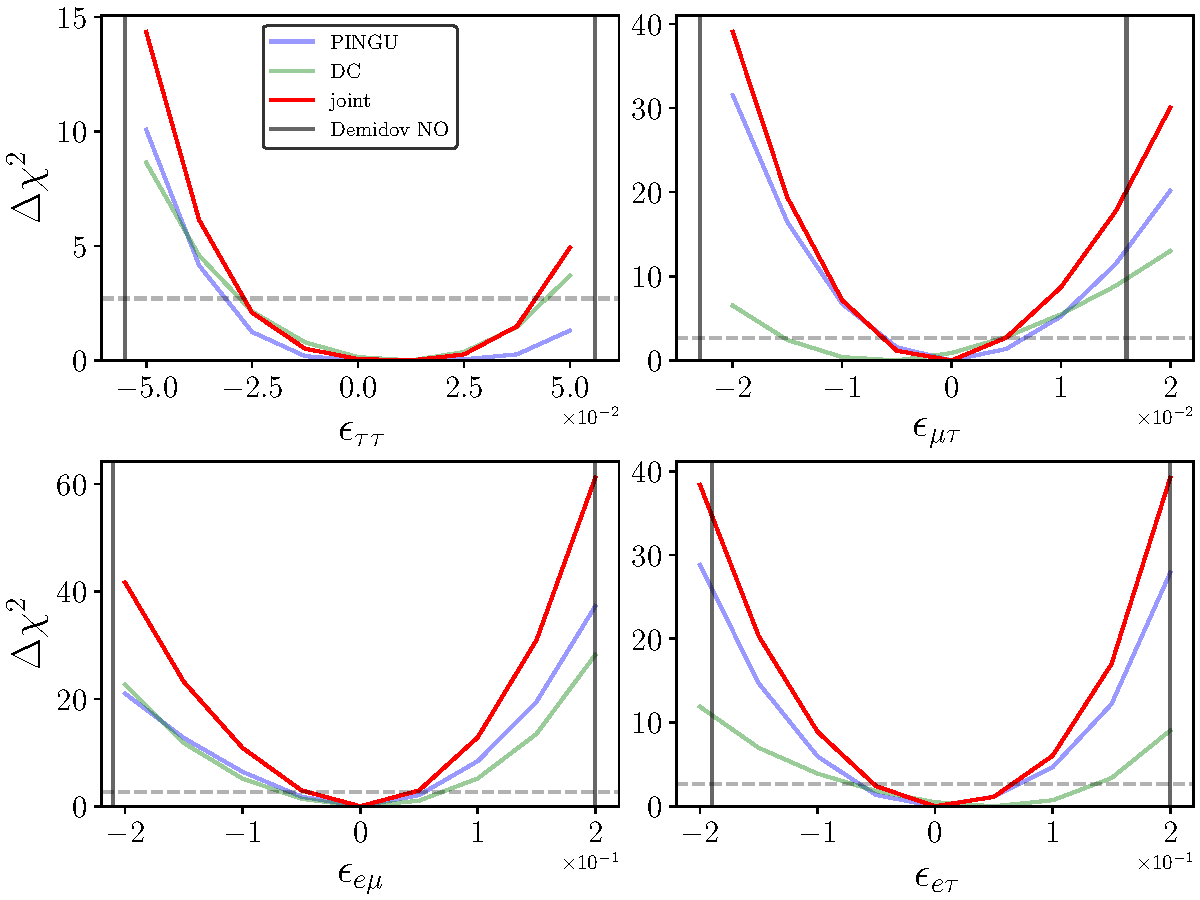
\includegraphics[scale = 0.7]{figures/joint_3D_NO.pdf}
      \caption{Confidence regions for PINGU and DeepCore scenarios listed in Table~\ref{table:syst_errors}, with their joint $\Delta \chi^2$ in maroon. $\dm[31]$ and $\theta_{23}$ and have been marginalized out, and all other NSI 
      parameters not shown in each panel are fixed to zero. 
      IceCube tracks only reveal $\emt$, and are displayed separately in Fig.~\ref{fig:IC_3D}. Dotted lines are the 90\% and $3\sigma$ CL levels.}\label{fig:3D_NO}
   \end{center}
\end{figure} 
\begin{figure}
   \begin{center} 
      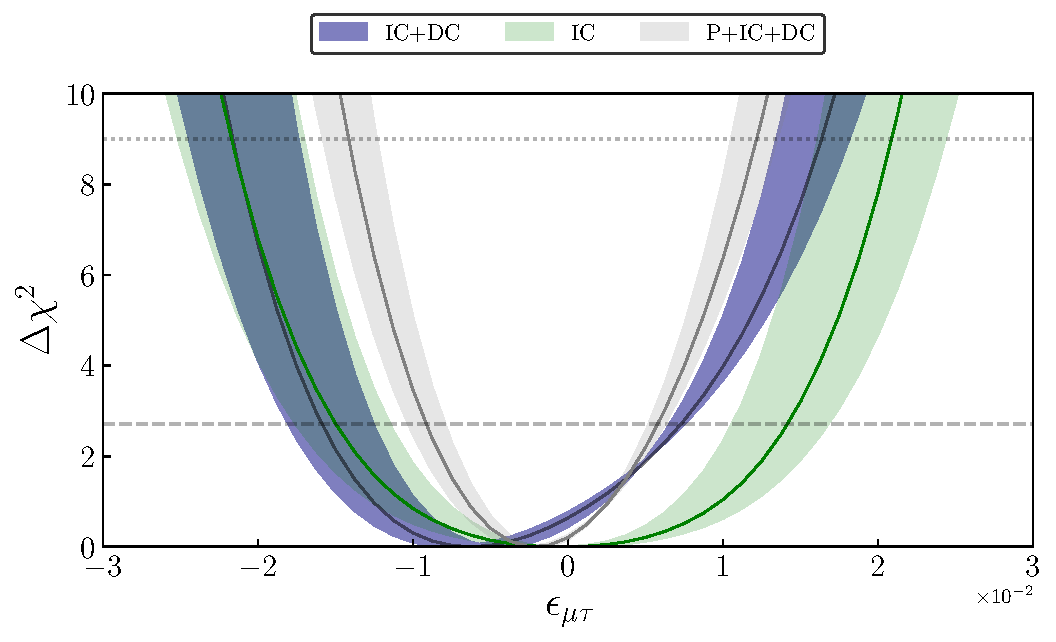
\includegraphics[width=0.8\textwidth]{figures/PID_3D_emt.pdf}
      \caption{IceCube $\emt$ $\Delta \chi^2$ regions for scenarios as defined in Table~\ref{table:syst_errors}.
    $\dm[31]$ and $\theta_{23}$ and have been marginalized out, and all other NSI 
    parameters other than $\emt$ are fixed to zero.Dotted lines are the 90\% and $3\sigma$ CL levels.}\label{fig:IC_3D}
   \end{center}
\end{figure}

%TODO: PINGU values are the same. Fill in empty values
{\renewcommand{\arraystretch}{1.0}
 \begin{table}
   \begin{center}
      \begin{tabular}{lcc}
         \hline
         Parameter & Best 90\% CL & Best $3\sigma$\\
         \hline & \multicolumn{2}{c}{IceCube}  \\
         $\emt$ &  [-0.008, 0.009] &  [-0.014, 0.017]  \\\\
         & \multicolumn{2}{c}{DeepCore}\\ [0.3em]
         $\ett$ &  [-0.044, 0.051] &  [-0.062, 0.069] \\
         $\emt$ &  [-0.008, 0.009] &  [-0.014, 0.017] \\
         $\eem$ &  [-0.079, 0.081] &   [-0.16, 0.14] \\
         $\eet$ &  [-0.079, 0.098] &  [-0.15, 0.16] \\\\
         &\multicolumn{2}{c}{IceCube + DeepCore} \\
         $\emt$ &  [-0.029, 0.007] &          [0.026] \\
         \hline
         \vspace{2em}
      \end{tabular}
      \begin{tabular}{lcc}
         \hline
         Parameter & Baseline 90\% CL & Baseline $3\sigma$ \\
         \hline & \multicolumn{2}{c}{IceCube}  \\
         $\emt$ &  [-0.009, 0.01] &  [-0.015, 0.018]  \\\\
         & \multicolumn{2}{c}{DeepCore}\\ [0.3em]
         $\ett$ &    [-0.046, 0.054] &         [-0.065]  \\
         $\emt$ &     [-0.009, 0.01] &  [-0.015, 0.018]  \\
         $\eem$ &  [-0.11, 0.094] &  [-0.20, 0.16]    \\
         $\eet$ &    [-0.10, 0.11] &  [-0.19, 0.18]  \\\\
         &\multicolumn{2}{c}{IceCube + DeepCore}\\
         $\emt$ &   [-0.029, 0.007] &          [0.026] \\
         \hline
         \vspace{2em}
      \end{tabular}
      \begin{tabular}{lcc}
         \hline
         Parameter & Worst 90\% CL & Worst $3\sigma$\\
         \hline & \multicolumn{2}{c}{IceCube}  \\
         $\emt$ &   [-0.01, 0.011] &   [-0.017, 0.02] \\\\
         & \multicolumn{2}{c}{DeepCore}\\ [0.3em]
         $\ett$ &    [-0.049, 0.057] &          [-0.07] \\
         $\emt$ &     [-0.01, 0.011] &   [-0.017, 0.02] \\
         $\eem$ &   [-0.14, 0.11] &   [-0.23, 0.18] \\
         $\eet$ &   [-0.13, 0.13] &  [-0.23, 0.12] \\\\
         &\multicolumn{2}{c}{IceCube + DeepCore}\\
         $\emt$ &   [-0.029, 0.007] &          [0.026] \\
         \hline
      \end{tabular}
      \caption{IceCube and DeepCore results from the $\Delta \chi^2$ in Fig.~\ref{fig:IC_3D}. $\dm[31]$ and $\theta_{23}$ have been marginalized out, and all other NSI parameters other than the one shown for each row are set to zero. Best, baseline, and worst refer to 
      the systematic uncertainty scenarios considered as in Table~\ref{table:syst_errors}.}\label{table:IC_DC_results}
   \end{center}
\end{table}

\begin{table}
   \centering
   \begin{tabular}{lcc}
      \hline
      Parameter & Best 90\% CL & Best $3\sigma$\\
      \hline & \multicolumn{2}{c}{PINGU} \\
      $\ett$ &  [-0.054, 0.067] &               [] \\
      $\emt$ &  [-0.029, 0.007] &          [0.026] \\
      $\eem$ &  [-0.12, 0.15] &  [-0.23, 0.24] \\
      $\eet$ &   [-0.084, 0.15] &  [-0.19, 0.21] \\\\
      & \multicolumn{2}{c}{DeepCore + PINGU} \\
      $\ett$ &  [-0.036, 0.046] &  [-0.056, 0.064] \\
      $\emt$ &  [-0.009, 0.006] &  [-0.015, 0.013] \\
      $\eem$ &   [-0.06, 0.077] &  [-0.126, 0.127] \\
      $\eet$ &  [-0.052, 0.095] &  [-0.112, 0.144] \\\\
      & \multicolumn{2}{c}{IceCube + DeepCore + PINGU}  \\
      $\emt$ &  [-0.009, 0.006] &  [-0.015, 0.013]  \\
      \hline
      %\vspace{0.5em}
   \end{tabular}
   \begin{tabular}{lcc}
      \hline 
      Parameter & Baseline 90\% CL & Baseline $3\sigma$\\
      \hline & \multicolumn{2}{c}{PINGU} \\
      $\ett$ &   [-0.054, 0.067] &               []\\
      $\emt$  &  [-0.029, 0.007] &          [0.026]  \\
      $\eem$ &    [-0.12, 0.15] &  [-0.23, 0.24] \\
      $\eet$ &    [-0.084, 0.15] &  [-0.19, 0.21] \\\\
      & \multicolumn{2}{c}{DeepCore + PINGU} \\
      $\ett$ &    [-0.038, 0.048] &  [-0.058, 0.067] \\
      $\emt$ &    [-0.01, 0.006] &  [-0.016, 0.014] \\
      $\eem$ &    [-0.071, 0.086] &  [-0.149, 0.141]  \\
      $\eet$ &   [-0.061, 0.103] &  [-0.131, 0.155] \\\\
      & \multicolumn{2}{c}{IceCube + DeepCore + PINGU}  \\
      $\emt$ &   [-0.01, 0.006] &  [-0.016, 0.014] \\
      \hline
      %\vspace{0.5em}
   \end{tabular}
   \begin{tabular}{lcc}
      \hline 
      Parameter & Worst 90\% CL & Worst $3\sigma$\\
      \hline & \multicolumn{2}{c}{PINGU} \\
      $\ett$ &    [-0.054, 0.067] &               [] \\
      $\emt$ &    [-0.029, 0.007] &          [0.026] \\
      $\eem$ &  [-0.12, 0.15] &  [-0.23, 0.24] \\
      $\eet$ &   [-0.084, 0.15] &  [-0.19, 0.21] \\\\
      & \multicolumn{2}{c}{DeepCore + PINGU} \\
      $\ett$ &     [-0.039, 0.05] &          [-0.06] \\
      $\emt$ &  [-0.011, 0.007] &  [-0.017, 0.015] \\
      $\eem$ &   [-0.082, 0.097] &  [-0.17, 0.16] \\
      $\eet$ &   [-0.067, 0.11] &  [-0.15, 0.17] \\\\
      & \multicolumn{2}{c}{IceCube + DeepCore + PINGU}  \\
      $\emt$ &   [-0.011, 0.007] &  [-0.017, 0.015] \\
      \hline
   \end{tabular}
   \caption{PINGU and joint results from the $\Delta \chi^2$ in Fig.~\ref{fig:3D_NO}. $\dm[31]$ and $\theta[23]$ have been marginalized out, and all other NSI parameters other than the one shown for each row are set to zero.
   Best, baseline, and worst refer to 
   the systematic uncertainty scenarios considered as in Table~\ref{table:syst_errors}.}\label{table:PINGU_joint_results}
\end{table}

%TODO: compare results, fix tables

\begin{table}
   \begin{center}
   \begin{tabular}{lccc}
           \hline \hline & \multicolumn{3}{c} {\text {Best fit}} \\
           \cline { 2 - 4 } Parameter & $\dm$ & $\theta_{23}$  & $\epsilon$  \\
           \hline \multicolumn{3}{c} {\hspace{2.5cm} DeepCore }  \\[0.1em]
           $\ett$ &  2.435 & 47.84 & 0.0125 \\
           $\emt$ &  2.435 & 43.97 & -0.005 \\
           $\eem$ &  2.435 & 43.97 & 0 \\
           $\eet$ &  2.435 & 43.97  & 0.05 \\\\
           \multicolumn{3}{c} {\hspace{2.5cm} IceCube } \\
           $\emt$ &  2.435 & 51.70 & 0 \\
           \multicolumn{3}{c} {\hspace{2.5cm} IceCube + DeepCore } \\
           $\emt$ &  2.517 & 43.97 & -0.01 \\
           \hline
           \hline
   \end{tabular}
   \end{center}
   \caption{Best fit points for $\dm[31]$ and $\theta_{23}$ are given in units of $\si{10^{-3}\eV\squared}$ and
   degrees, respectively.}\label{table:bestfit}
\end{table}
\newpage


 \begin{figure}[t]
   \begin{center}
      \begin{subfigure}{0.47\textwidth}
         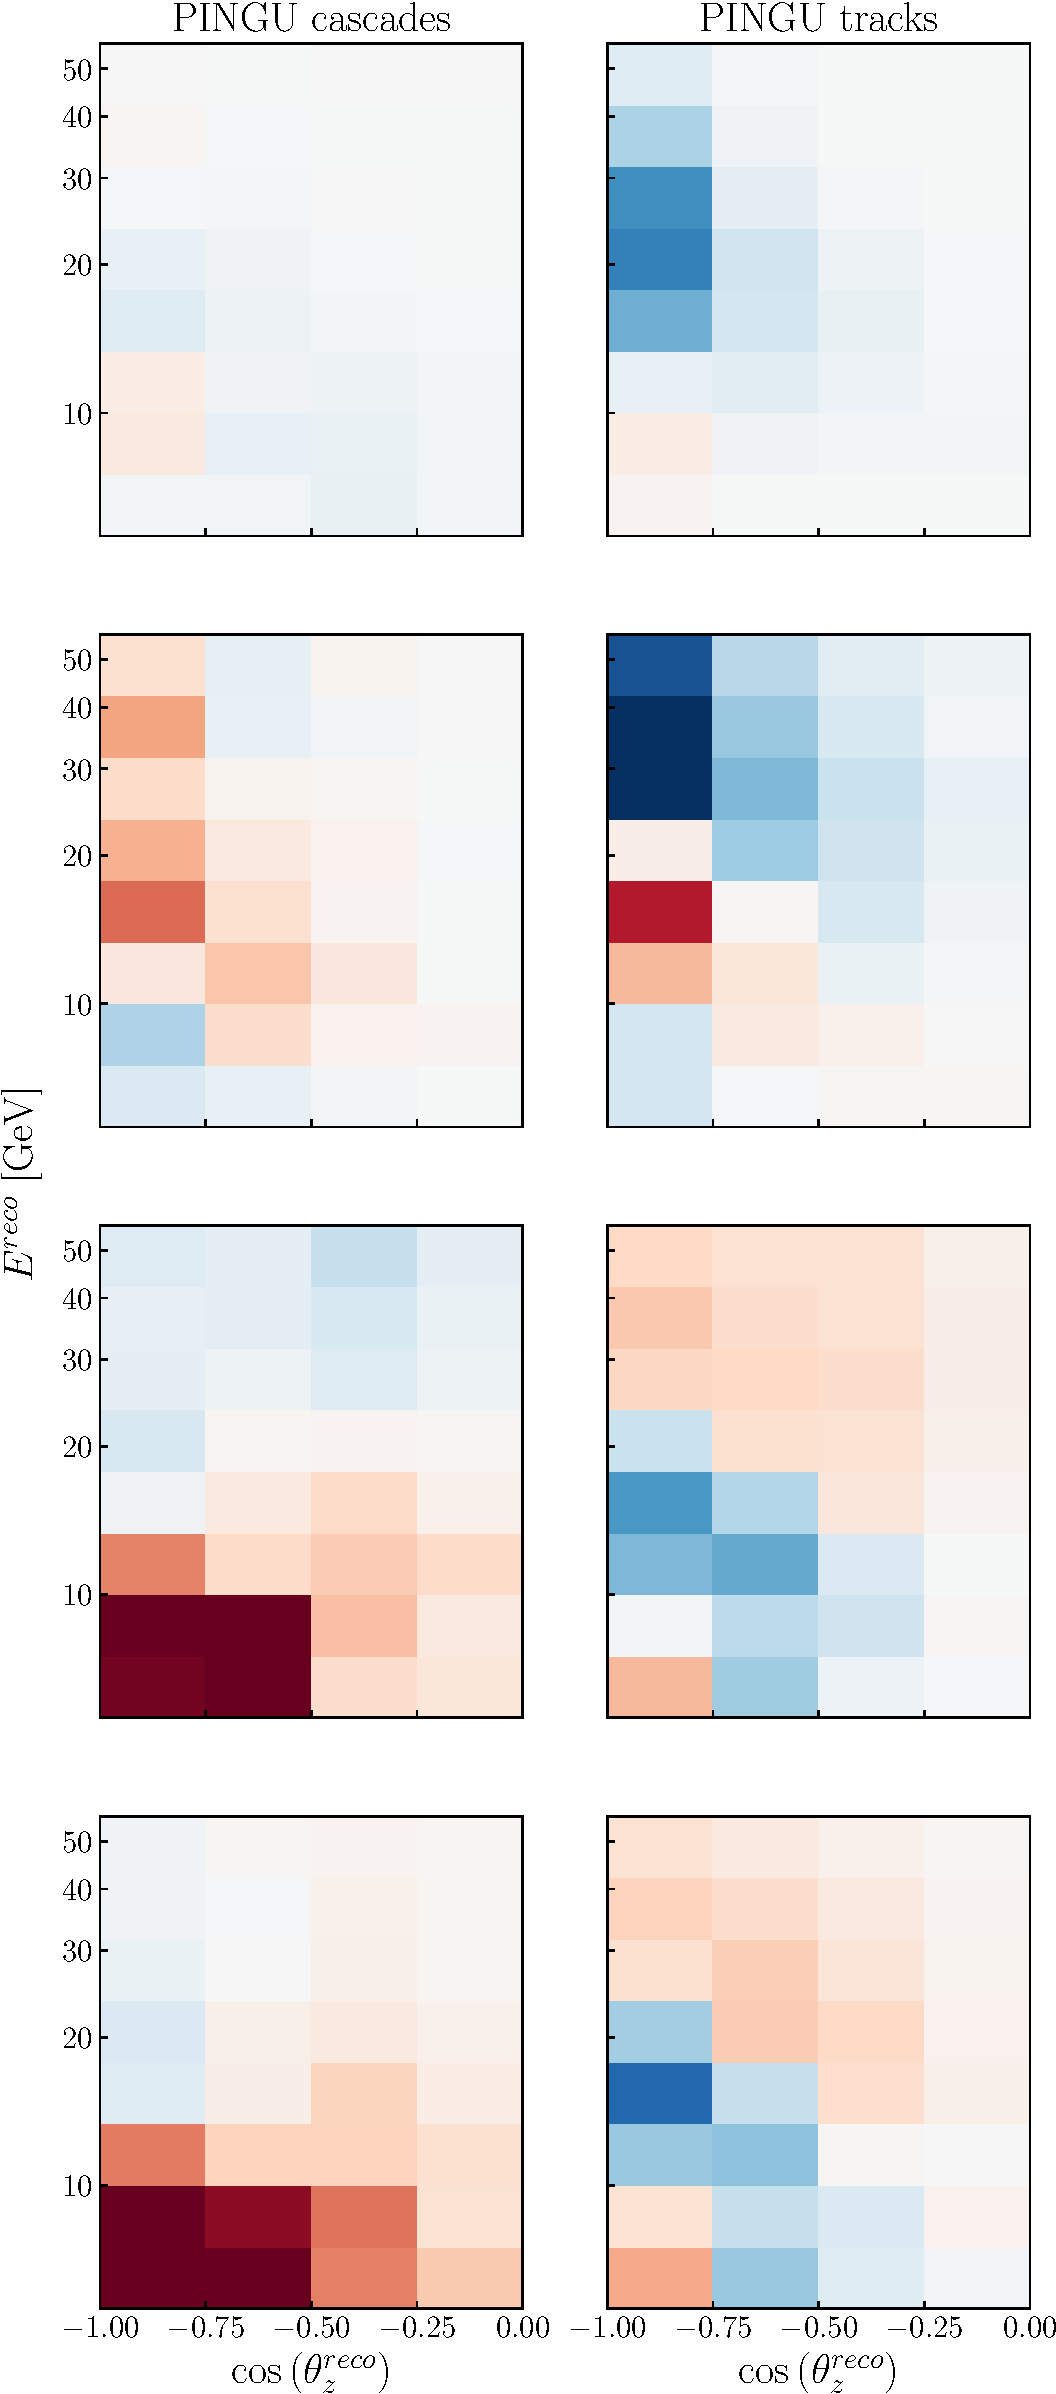
\includegraphics[width=1\linewidth]{figures/PINGU_event_pulls.pdf}
         \caption{PINGU}\label{fig:PINGU_event_pulls}
      \end{subfigure}
      \begin{subfigure}{0.51\textwidth}
         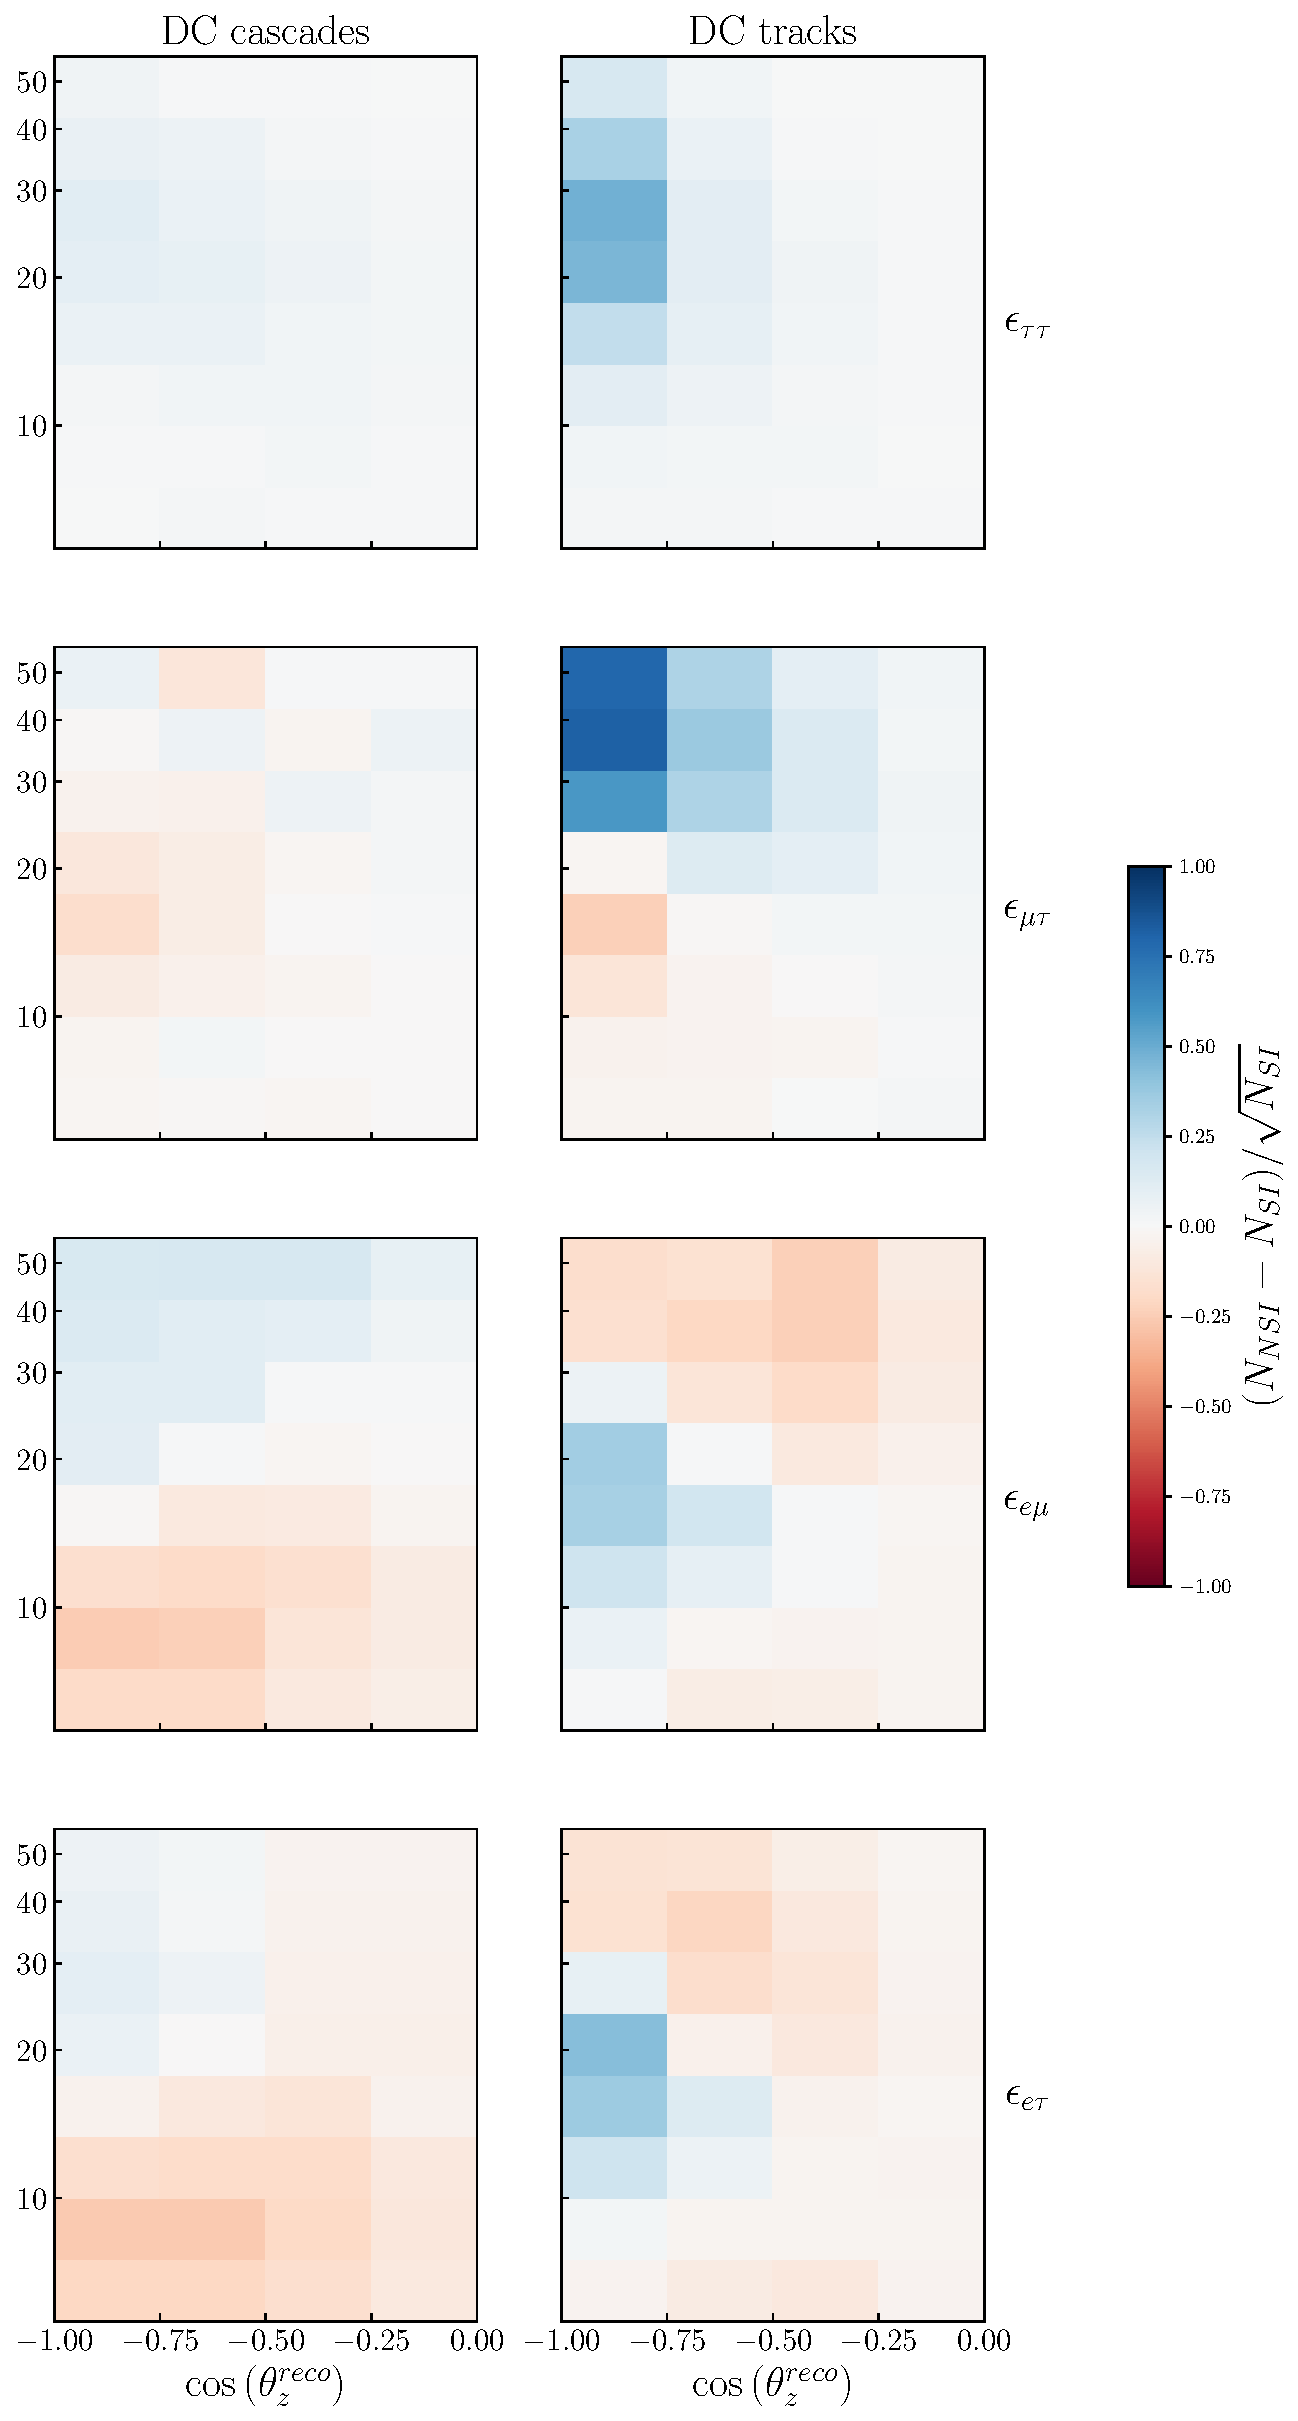
\includegraphics[width=1\linewidth]{figures/DC_event_pulls.pdf}
         \caption{DeepCore}\label{fig:DC_event_pulls}
      \end{subfigure}
    \end{center}
   \caption{Expected pulls of the form $(N_{NSI} - N_{SI})/\sqrt{N_{SI}}$ for PINGU and DeepCore after 3 years.}
\end{figure}
%TODO 5.6 is small, fix labels
There is no reason for us to assume that only one NSI parameter exists in Nature, unless we impose a symmetry on the gauge group which generates NSI. For example, the matter potential matrix in our Hamiltonian from Eq.~\eqref{eq:V_matrix} is diagonal since the interaction Lagrangian respects lepton number conservation. 
The PMNS matrix, on the other hand, has off-diagonal elements because the kinetic Lagrangian breaks this symmetry. So ideally, we would simulate a grid where all NSI parameters are allowed to vary, 
but this is not feasible. Thus, we take we set $\ett = 0$ and let $\emt,\eem,\eet$ vary, along with $\dm[31]$ and $\theta_{23}$. We let $\ett=0$ because we saw that it did not influence the other parameters. 
We then marginalize out the standard oscillation parameters and one of the NSI parameters and plot the remaining two in Fig.~\ref{fig:PINGU_2D}. We see that the pairs $\eem - \emt$ and $\eet - \emt$ are symmetrical. 
Hence, we can see that no relationship exists between them. With $\eet - \eem$, however, the contours are assuming a different shape. The contour allows positive values of $\eet$ and $\eem$ to a greater degree than mixed or negative values.
Thus, we can draw the conclusion that, given $\ett = 0$, PINGU might expect to observe that $\eem$ and $\emt$ are anti-correlated while we expect no significant correlation
to be be seen between the pairs $\emt - \eem$, and $\emt - \eet$.

\begin{figure}
   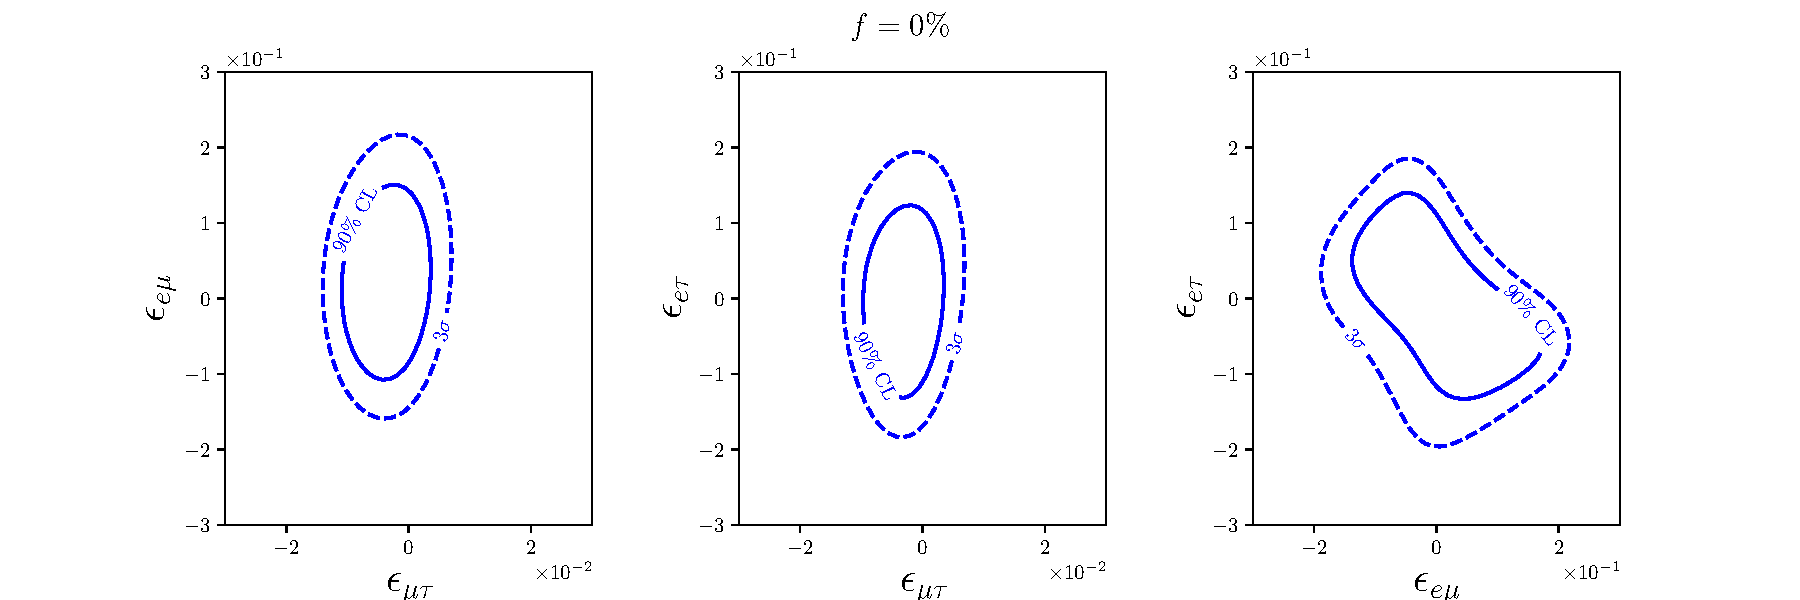
\includegraphics[scale=0.5]{figures/PINGU_2D_all_f0.pdf}
   \caption{Allowed regions for some of the NSI parameters after three years of PINGU data, assuming no uncorrelated systematic error. All plots are made with $\ett = 0$. The two
   standard oscillation parameters $\dm[31]$ and $\theta_{23}$ along with the one NSI parameter not shown have been marginalized out. The values of the standard oscillation parameters 
   are taken from NuFit~\cite{nufit}.}\label{fig:PINGU_2D}
\end{figure}